\usepackage[utf8]{inputenc}
\usepackage[T1]{fontenc}
\usepackage{textcomp}

\usepackage{url}

\usepackage[
    sorting=nyt,
    style=alphabetic
]{biblatex}
\addbibresource{bibliography.bib}

\usepackage{hyperref}
\hypersetup{
    colorlinks,
    linkcolor={black},
    citecolor={black},
    urlcolor={blue!80!black}
}
\usepackage[noabbrev]{cleveref}

% Adds Bibliography, ... to Table of Contents
\usepackage[nottoc]{tocbibind}

\usepackage{graphicx}
\usepackage{float}
\usepackage[usenames,dvipsnames,svgnames]{xcolor}

% \usepackage{cmbright}

\usepackage{amsmath, amsfonts, mathtools, amsthm, amssymb}
\usepackage{mathrsfs}
\usepackage{cancel}

\newcommand\N{\ensuremath{\mathbb{N}}}
\newcommand\R{\ensuremath{\mathbb{R}}}
\newcommand\Z{\ensuremath{\mathbb{Z}}}
\renewcommand\O{\ensuremath{\emptyset}}
\newcommand\Q{\ensuremath{\mathbb{Q}}}
\newcommand\C{\ensuremath{\mathbb{C}}}
\let\implies\Rightarrow
\let\impliedby\Leftarrow
\let\iff\Leftrightarrow
\let\epsilon\varepsilon

\usepackage{tikz}
\usepackage{tikz-cd}

% theorems
\usepackage{thmtools}
\usepackage{thm-restate}
\usepackage[framemethod=TikZ]{mdframed}
\mdfsetup{skipabove=1em,skipbelow=0em, innertopmargin=12pt, innerbottommargin=8pt}

\theoremstyle{definition}

\makeatletter

\declaretheoremstyle[headfont=\bfseries\sffamily, bodyfont=\normalfont, mdframed={ nobreak } ]{thmgreenbox}
\declaretheoremstyle[headfont=\bfseries\sffamily, bodyfont=\normalfont, mdframed={ nobreak } ]{thmredbox}
\declaretheoremstyle[headfont=\bfseries\sffamily, bodyfont=\normalfont]{thmbluebox}
\declaretheoremstyle[headfont=\bfseries\sffamily, bodyfont=\normalfont]{thmblueline}
\declaretheoremstyle[headfont=\bfseries\sffamily, bodyfont=\normalfont, numbered=no, mdframed={ rightline=false, topline=false, bottomline=false, }, qed=\qedsymbol ]{thmproofbox}
\declaretheoremstyle[headfont=\bfseries\sffamily, bodyfont=\normalfont, numbered=no, mdframed={ nobreak, rightline=false, topline=false, bottomline=false } ]{thmexplanationbox}

\declaretheoremstyle[headfont=\bfseries\sffamily, bodyfont=\normalfont, numbered=no, mdframed={ nobreak, rightline=false, topline=false, bottomline=false } ]{thmexplanationbox}


\declaretheorem[numberwithin=chapter, style=thmgreenbox, name=Definition]{definition}
\declaretheorem[sibling=definition, style=thmredbox, name=Corollary]{corollary}
\declaretheorem[sibling=definition, style=thmredbox, name=Proposition]{prop}
\declaretheorem[sibling=definition, style=thmredbox, name=Theorem]{theorem}
\declaretheorem[sibling=definition, style=thmredbox, name=Lemma]{lemma}
\declaretheorem[sibling=definition, style=thmbluebox,  name=Example]{eg}
\declaretheorem[sibling=definition, style=thmbluebox,  name=Nonexample]{noneg}
\declaretheorem[sibling=definition, style=thmblueline, name=Remark]{remark}




\declaretheorem[numbered=no, style=thmexplanationbox, name=Proof]{explanation}
\declaretheorem[numbered=no, style=thmproofbox, name=Proof]{replacementproof}
\declaretheorem[style=thmbluebox,  numbered=no, name=Exercise]{ex}
\declaretheorem[style=thmblueline, numbered=no, name=Note]{note}

% \renewenvironment{proof}[1][\proofname]{\begin{replacementproof}}{\end{replacementproof}}

% \AtEndEnvironment{eg}{\null\hfill$\diamond$}%

\newtheorem*{uovt}{UOVT}
\newtheorem*{notation}{Notation}
\newtheorem*{previouslyseen}{As previously seen}
\newtheorem*{problem}{Problem}
\newtheorem*{observe}{Observe}
\newtheorem*{property}{Property}
\newtheorem*{intuition}{Intuition}


\declaretheoremstyle[
    headfont=\bfseries\sffamily\color{RawSienna!70!black}, bodyfont=\normalfont,
    mdframed={
        linewidth=2pt,
        rightline=false, topline=false, bottomline=false,
        linecolor=RawSienna, backgroundcolor=RawSienna!5,
    }
]{todo}
\declaretheorem[numbered=no, style=todo, name=TODO]{TODO}


\usepackage{etoolbox}
\AtEndEnvironment{vb}{\null\hfill$\diamond$}%
\AtEndEnvironment{intermezzo}{\null\hfill$\diamond$}%

% http://tex.stackexchange.com/questions/22119/how-can-i-change-the-spacing-before-theorems-with-amsthm
% \def\thm@space@setup{%
%   \thm@preskip=\parskip \thm@postskip=0pt
% }

\usepackage{xifthen}

\makeatother

% figure support (https://castel.dev/post/lecture-notes-2)
\usepackage{import}
\usepackage{xifthen}
\pdfminorversion=7
\usepackage{pdfpages}
\usepackage{transparent}


\makeatletter
\newif\ifworking
\@ifclasswith{tuftebook}{working}{\workingtrue}{\workingfalse}
\makeatother

\newcommand{\incfig}[2][1]{%
    % \ifworking{\makebox[0pt][c]{\color{gray}{\scriptsize\textsf{#2}}}}\fi%
    \def\svgwidth{#1\textwidth}
    \import{./figures/}{#2.pdf_tex}
}

\newcommand{\fullwidthincfig}[2][0.90]{%
    % \ifworking{\makebox[0pt][l]{\color{gray}{\scriptsize\textsf{#2}}}}\fi%
    \def\svgwidth{#1\paperwidth}
    \import{./figures/}{#2.pdf_tex}
}



\newcommand{\minifig}[2]{%
    \def\svgwidth{#1}%
    \begingroup%
    \setbox0=\hbox{\import{./figures/}{#2.pdf_tex}}%
    \parbox{\wd0}{\box0}\endgroup%
    \hspace*{0.2cm}
}

% %http://tex.stackexchange.com/questions/76273/multiple-pdfs-with-page-group-included-in-a-single-page-warning
\pdfsuppresswarningpagegroup=1

\newcommand\todo[1]{\ifworking {{\color{red}{#1}}} \else {}\fi}
\newcommand\charlotte[1]{\ifworking {{\color{blue}{#1}}} \else {}\fi}

\author{Gilles Castel}



\usepackage{multirow}
\def\block(#1,#2)#3{\multicolumn{#2}{c}{\multirow{#1}{*}{$ #3 $}}}

% \overfullrule=1mm

\newenvironment{myproof}[1][\proofname]{%
  \proof[\rm \bf #1]%
}{\endproof}

\title{\vspace{-1cm}Pendul\vspace{-1cm}}
\author{}
\date{}

\usepackage{multicol}
\begin{document}
\maketitle
\thispagestyle{fancy}
\begin{figure}[ht]
    \centering
    \incfig{pendul}
    \caption{pendul}
    \label{fig:pendul}
\end{figure}
\begin{figure}[ht]
    \centering
    \incfig{pendul2}
    \caption{pendul2}
    \label{fig:pendul2}
\end{figure}
\begin{subexercise}{Pendul uden friktion, lille vinkel}

\end{subexercise}
\begin{solution}
Hvis vi antager at friktionskraften er $0$. Vil der kun være én kraft på pendulet,
 \[
F = m\cdot g\cdot \sin \theta
.\]
Kraftmomentet på pendulet vil være afstanden fra pivot-punktet til center of mass ganget med den vinkelrette komponent af kraften. 
\[
	\tau = -(mg)\sin \theta \cdot R_{cm}
.\] 
Hvis jeg nu også laver en lille-vinkel antagelse,
\[
	\tau = -(mg) \cdot \theta \cdot R_{cm}
.\]
Jeg ved desuden at kraftmomentet er,
\[
	I \frac{\dd^2 \theta}{\dd t^2} = -(mg)\cdot \theta(t)\cdot  R_{cm}
.\] 
 Vi vil gerne finde en funktion $\theta(t)$, som opfylder denne ligning. Jeg betrager funktionen $\theta (t) = \frac{1}{I}\cdot \sin(t\cdot \sqrt{mgR_{cm}}+\lambda )+c$.
\begin{align*}
	\frac{\dd \theta^2}{\dd t^2} \theta (t) &= \frac{\dd \theta}{\dd t}\frac{1}{I}\cdot \sqrt{mgR_{cm}}\left( -\cos(t\cdot \sqrt{mgR_{cm}} +\lambda \right)  \\
						&= \frac{-mgR_{cm}}{I}\sin(t\cdot \sqrt{mgR_{cm}} +\lambda) \\
.\end{align*}
Og ser at denne funktion opfylder kriteriet. I en analyse $\sin(t)$ ser jeg at $\sin(t) = t$ approksimationen holder nogenlunde for vinkler mindre end $0.40$ radianer.
\end{solution}

\begin{subexercise}{Pendul med friktion, lille vinkel}

\end{subexercise}
\begin{solution}
Hvis vi nu antager at der yderligere er en friktionskraft som påvirker pendulet, ændres situation. Det er en rimelig antagelse at denne friktionskraft er proportionel med pendulets hastighed.
\[
F_k = -b\cdot v = -b\cdot \omega R_{cm} 
.\] 
Kraftmomentet den giver anledning til er så,
\[
\tau_k = -b \cdot \omega \cdot R_{cm}^2
.\]
Det totale kraftmoment bliver da,
\[
	\tau_{res} = I \frac{\dd^2 \theta}{\dd t^2} = -(mg)\cdot \theta (t) \cdot R_{cm} - b\cdot \frac{\dd \theta}{\dd t} \cdot R_{cm}^2
.\]
Denne differentialligning løses af funktionen,
\[
	\theta (t) = A\cdot \exp\left( \frac{-bR_{cm}^2t}{2I}\right)\cos(\omega t+ \phi)
.\] 
Hvor,
\[
\omega = \sqrt{\frac{R_{cm}mg}{I}- \left( \frac{bR_{cm}^2}{2I} \right) ^2} 
.\]
Vi ser her at friktionskraften, giver anledning til en faldende amplitude, og at vinkelfrekvensen dog stadig konstant, er mindre end den ville have været uden friktionskraften til stede.
\end{solution}
\begin{figure}[ht]
    \centering
    \incfig{massemidtpunkts_bestemmelse}
    \caption{Massemidtpunkt}
    \label{fig:massemidtpunkt}
\end{figure}
\newpage
\begin{subexercise}{Bestemmelse af massemidtpunktet}
Her følger de teoretiske overvejelse, til bestemmelse af pendulets massemidtpunkt.
\end{subexercise}\newline
Se figur 3. Der er 2 krafter på pendulet, en tension fra snoren og tyngdekraften. Tyngdekraften virker i pendulets massemidtpunkt, mens tension virker der hvor snoren sidder fast. Disse giver begge anledning til et kraftmoment, men da pendulet er i hvile vil det samlede kraftmoment være 0.
\[
\tau = F_wR_w + F_TR_T
.\] 
Nu definerer jeg $R_T = R_0 + \Delta R$
\begin{align*}
	\frac{1}{F_T}&= \frac{-\left( R_0+\Delta R \right) }{R_wF_w} \\
	\frac{1}{F_T}&= \frac{-R_0}{R_wF_w}-\frac{\Delta R}{R_wF_w}
.\end{align*}
\begin{subexercise}{Fejlpropagering, bestemmelse af perioder og skalering}

\end{subexercise}
\begin{solution}
Som del af forsøget, vælger vi at kigge på sammenhængen mellem maks-amplituden og perioden. Vi formoder at der er en relation ala,
\[
	T(\theta_{maks}) = T_0 \cdot f(\theta_{maks})
.\]
Hvis der kun tages højde for tyngdekraften, kan $T_0$ udledes til at være lig,
\[
T_0 = 2\pi \sqrt{\frac{I_p}{M_pgL_p}} 
.\]
Dette er dog ikke sandt, i vores situation hvor der er gnidning i systemet. Vi vælger derfor i stedet at approksimere $T_0$ som værende perioden på den mindste målelige vinkeludsvinging. Dette er i vores tilfælde ca. 3 grader. Vores mål er nu, at se om der gælder en lignende mellem denne "eksperimentelle $T_0$" og perioden for større vinkel udsvingninger.
\subsubsection*{Usikkerhed forbundet med at bestemme perioden.}
Vi har valgt at bestemme usikkerheden på følgende måde: Perioden må givetvis være den tidslige afstand mellem 2 maksimale ekstrema i vores data. Vi har derfor skrevet et stykke kode som finder disse maksima. Der er dog her et lille problem. Pga. af opløsningen af vores data, kan der lokalt være flere punkter som har maksimale værdi. Det er dermed tvetydigt, hvilket af disse punkter, der er det egentlige toppunkt på kurven.\\
Vi har valgt at løse det ved at vælge det midterste punkt som toppunktet, og sige at usikkerheden på dette punkt er halvdelen af bredden af de mulige toppunkter.
\columnbreak
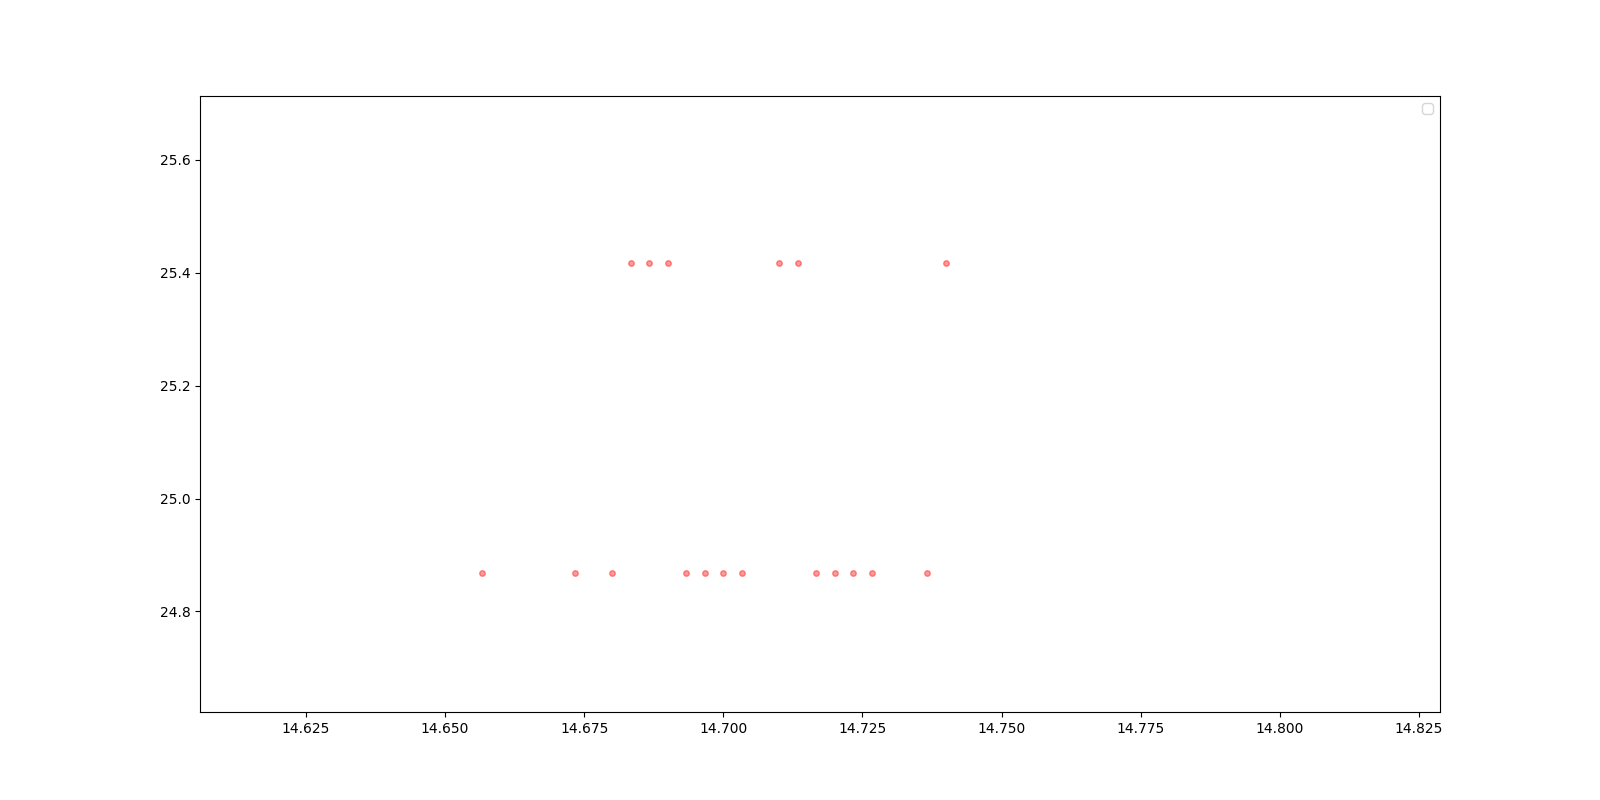
\includegraphics[width=0.5\textwidth]{../toppunkt1}
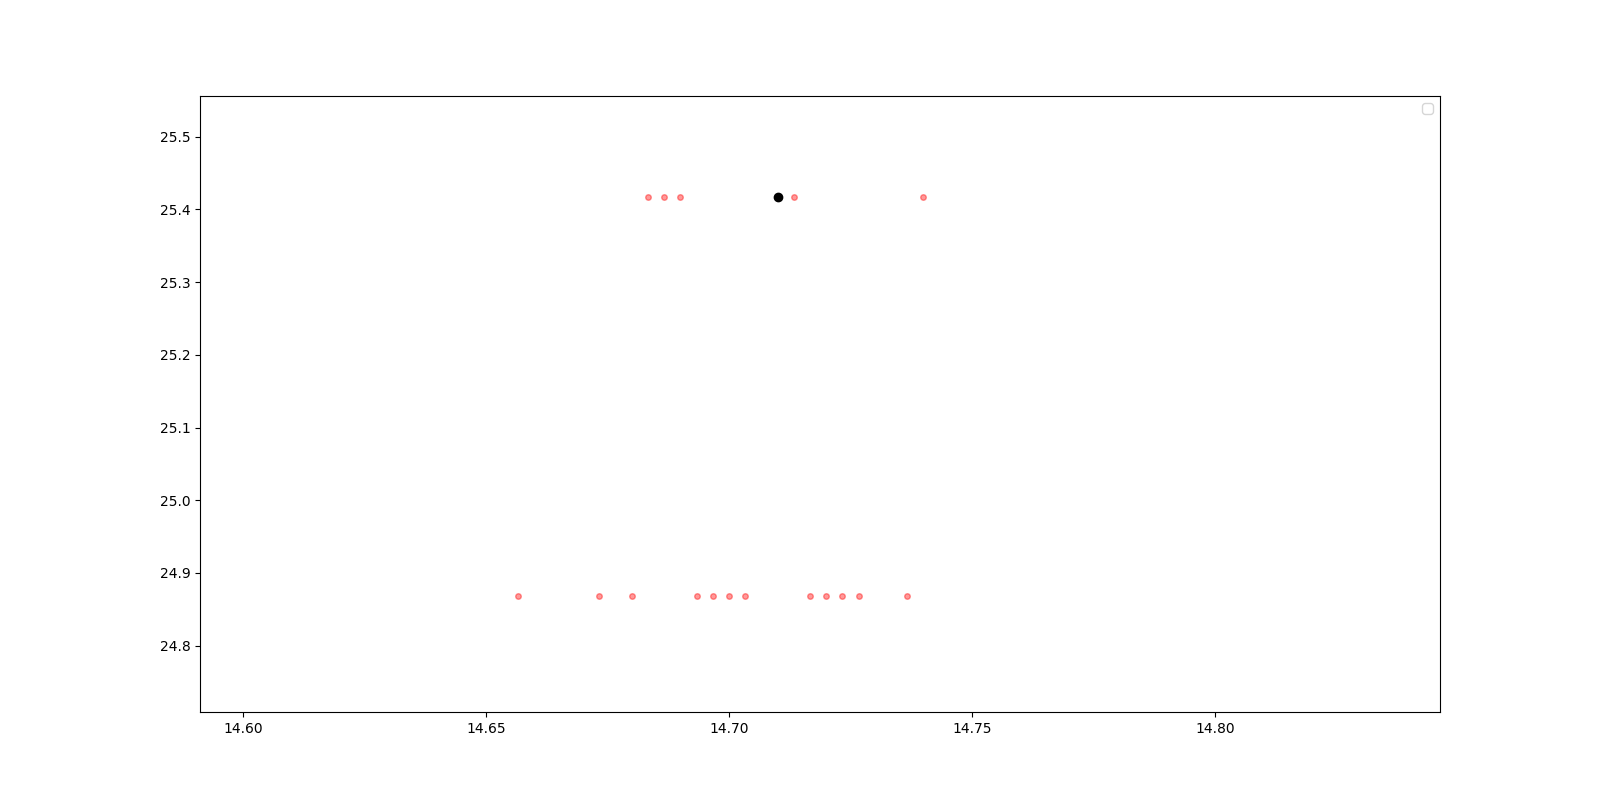
\includegraphics[width=0.5\textwidth]{../toppunkt2}
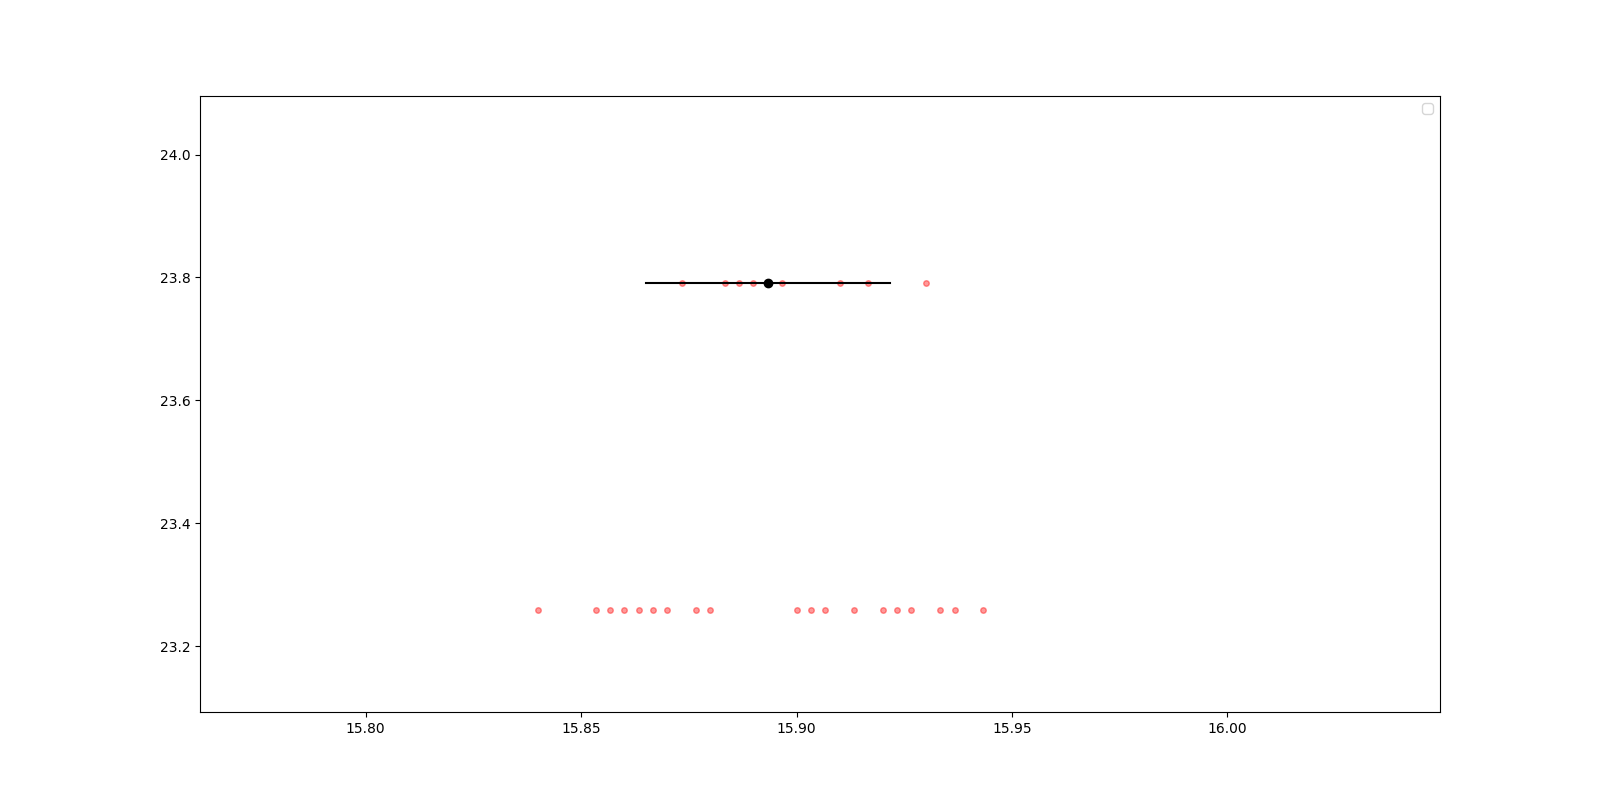
\includegraphics[width=0.5\textwidth]{../toppunkt3}
For at fitte til modellen, sætter vi $T_0 = 1$. Vi skalere derefter vores perioder til at følge med.
 \[
T_{scaled} = T\left( \theta \right) / T_0
.\] 
Alle disse perioder er fundet ud fra toppunkter som har en usikkerhed associeret med sig. Vi skal derfor lave fejlpropagering for at finde usikkerheden på $T_{scaled}$ 
\[
T_{scaled} = \frac{t_2-t_1}{t_0_2 - t_0_1}
.\]
Disse værdier har hver en usikkerhed associeret med sig. Vi betragter en funktion på formen,
\[
Z = \frac{A-B}{C-D}
.\] 
\[
\alpha _Z^2 =  \left| \frac{\dd Z}{\dd A}\right|^2\alpha _A^2 +\left| \frac{\dd Z}{\dd B}\right|^2\alpha _B^2+ \left| \frac{\dd Z}{\dd C}\right|^2\alpha _C^2+\left| \frac{\dd Z}{\dd D}\right|^2\alpha _D^2
.\] 
\end{solution}
Som udregnes,
\[
	\alpha _Z^2 = \frac{\alpha _A^2 + \alpha _B^2}{(C-D)^2}+\left| \frac{\dd Z}{\dd C}\right|^2\alpha _C^2+\left| \frac{\dd Z}{\dd D}\right|^2\alpha _D^2
.\]
\[
	\frac{\dd Z}{\dd C} = \left( A - B \right) \cdot \frac{1}{(C-D)^2} = - \frac{\dd Z}{\dd D}
.\] 
\[
	\left( \frac{\dd Z}{\dd C} \right) ^2 = \left( \frac{\dd Z}{\dd D} \right) ^2 = \left( A - B \right) ^2 \cdot \ln \left( C-D \right) ^2
.\] 
Dette kobles sammen til,
\[
\alpha _Z^2 = \frac{\alpha _A^2+\alpha _B^2}{\left( C-D \right) ^2} + \left( A-B \right) ^2\cdot \ln\left( C-D \right) ^2\left( \alpha _C^2 + \alpha _D^2 \right) 
.\]
Som altså er variansen på $Z$. 

\end{document}
